\section{Introduction}

Internet has enabled billions of people around the world to connect, cooperate, and communicate. However, even the most widely spoken language, Mandarin, is only spoken by 12\% of the world population. 
Other official languages of the United Nations, like English and French, are only spoken by 4.8\% and 1.0\% of the world, respectively \cite{Britannica Encyclopedia, http://www.britannica.com/EBchecked/topic/329791/language/292862/Most-widely-spoken-languages}. 
Even if we include non-native speakers who are able to communicate in that language, they still only represent 12\% and 3\% of the world, respectively \cite{http://en.wikipedia.org/wiki/List_of_languages_by_total_number_of_speakers, http://www.diplomatie.gouv.fr/en/french-foreign-policy-1/promoting-francophony/the-status-of-french-in-the-world/}. This means that even for someone who speaks two of the most popular languages in the world, English and French, the person is only able to communicate with a small percentage of the world population.

To understand how language barriers affect cooperative gaming experience over the Internet, we conducted a 12-person user study with 3 popular online cooperative games. We collected participants' experience and rating using extended Short Feedback Questionnaire (eSFQ) \cite{eSFQ} and Cooperative Performance Metrics (CPMs) \cite{CPMs}, and conducted interviews. Results showed that while none of the participants with common languages reported the games as frustrating, up to 67\% of the participants without common languages found the games frustrating. Also, participants without common languages rated fun and enjoyment significantly lower at 3.6 vs 4.3 (on a scale of 1 to 5) compared to the participants with common languages. 

%
%Consist of human communication, there are not only speech but also inclusive of various gestures and body motions. Body lan- guage, a non-verbal way to transmit your thoughts without verbal- izing. According to The 7% Rule[21], the influence for communi- cation for verbal is only 7% but is 93% for non-verbal expression. And the non-varbal expression is made up of body language (55%) and tones of voice (38%).
%Charades[3] is a word guessing game. It is an acting game in which one player acts as a word or a phrase, and sometime imitates a similar pronounced words, while the other players guess for the answer. The main idea is to use body to make physical expression rather than using verbal language.
%Inspired by The 7% Rule and the Charades, we suggested to use body language as a communication manner in cooperative game to normalize player’s communication skill. With this idea, whether players are playing with different language speakers or not, their communication skill is near enough for game developer to design a proper difficulty to entertain players. On the other hand, many re- searchers have argued that body movement brings about a positive emotional and social response [7, 10, 16]. We think that body lan- guage communication should enhance game engagement and en- joyment.
%

Nowadays, it is common for players to play cooperative games from different country under highly developed Internet environment. 
In our pilot study, we observed that playing cooperative game, which required high-level-feature communication, with different language speaker would cause frustrating game experience.

We suggest to use body language as a communication manner in cooperative game to get better game experience. With this approach, no matter playing with different language speaker or common language speaker, player would have consistent game experience. 

We also provide a game prototype, Mute Robot, to explore cooperative game design through body language. Mute Robot provides three game stages for players to solve puzzles.
To encourage players to use body language, we have designed an asymmetric puzzle system, with only one player receiving puzzle hints. The player will use body language to guide the other player to solve the puzzle.

By using extended Short Feedback Questionnaire (eSFQ)\cite{eSFQ} and Cooperative Performance Metrics (CPMs)\cite{CPMs} to evaluate game experience, our user study results indicate that, using body language in cooperative game design would enhance original game experience and decrease 48\% frustrating caused by language boundary. And we observe that cooperative game has consistent game experience with body language communication.

% According to our final questionnaire, only 17\% and 25\% (different language group and common language group) player choose traditional communication manner (speaking) as the favorite manner.
According to our final questionnaire, after adding the communication manner of body language, 83\% and 75\% (different language group and common language group) players choose our new communication manner (``body language'' and ``both'') as the favorite manner. 

We also observe some interesting communication patterns. Game developer can make a better game experience with these information. We hope to inspire more exploration of using body language in game designs and spread game entertainment for more people.


\begin{figure}[t]
\centering
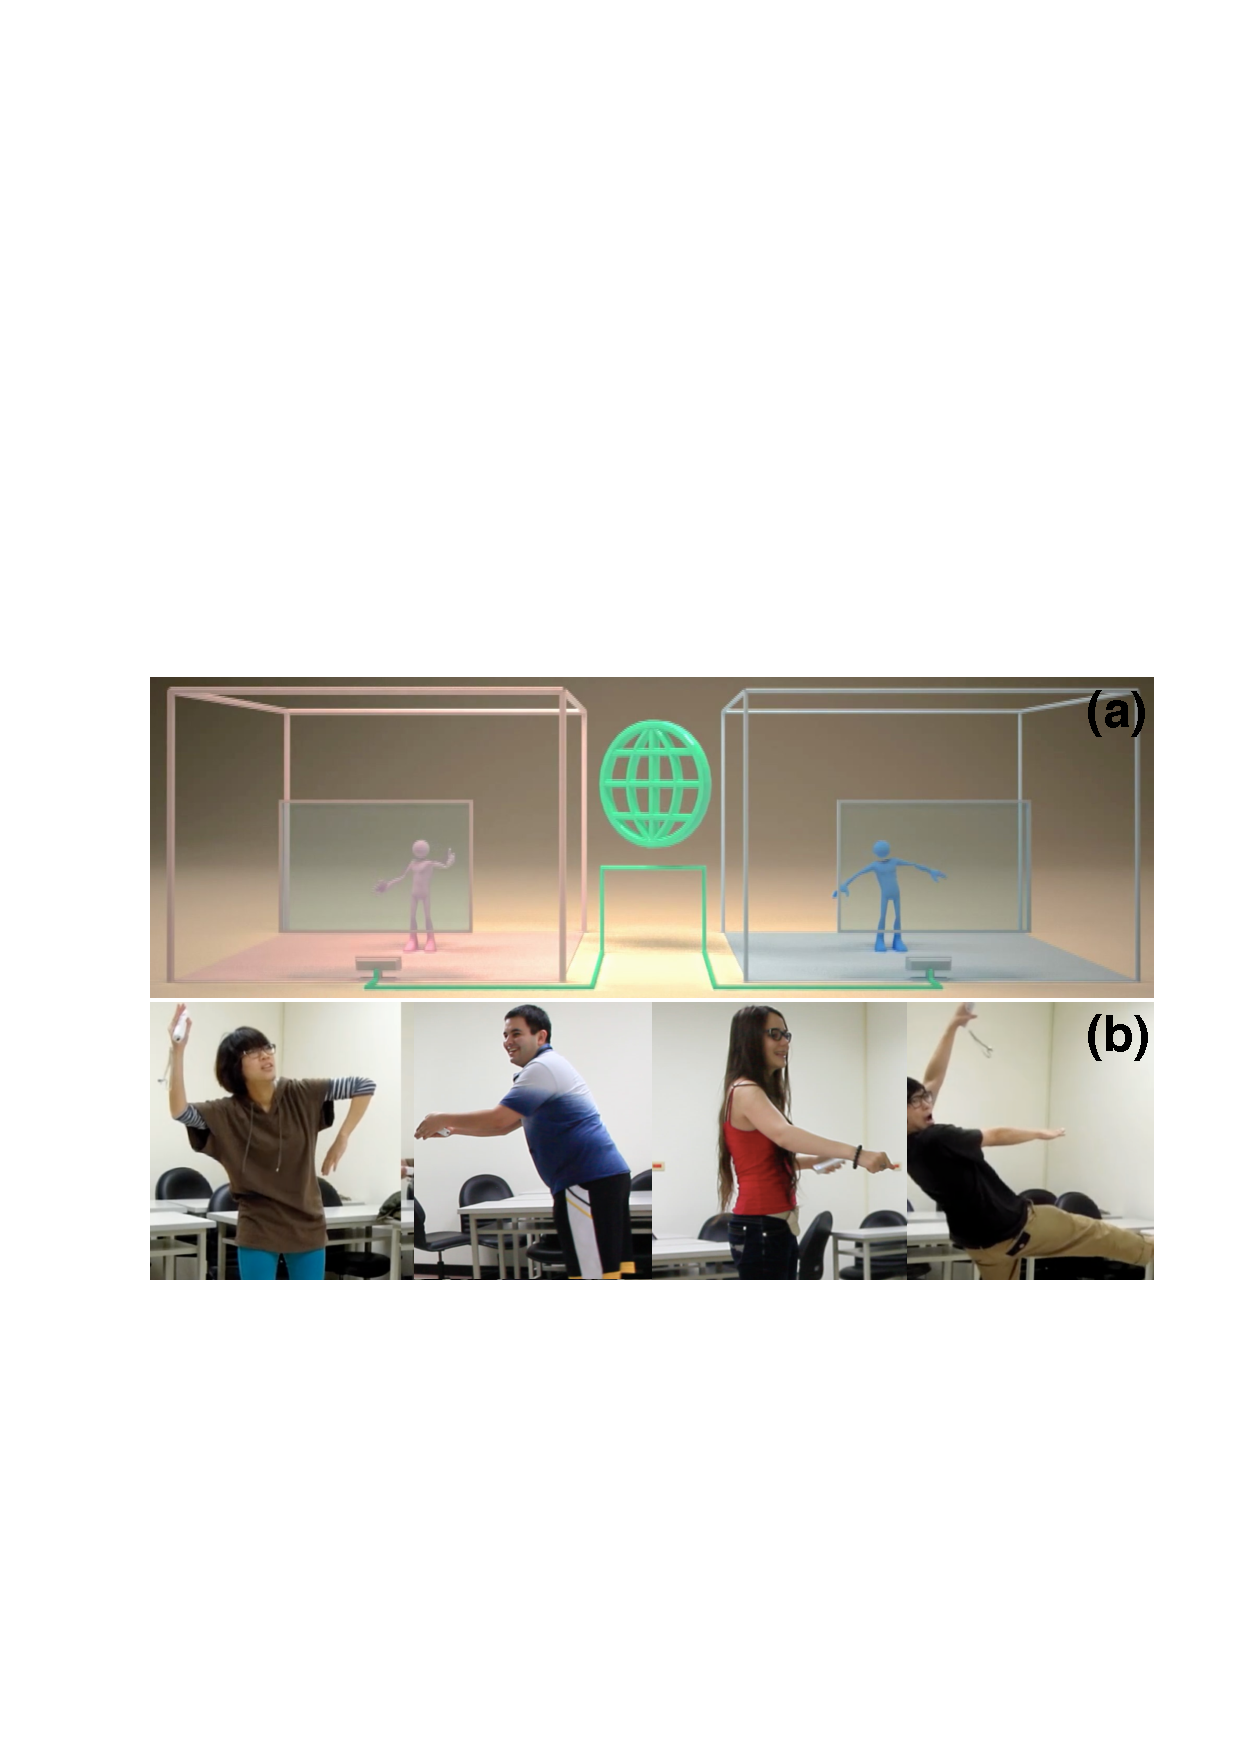
\includegraphics[width=0.9\columnwidth]{Figures/Topic.pdf}
\caption{(a) Playing cooperative games via Internet, (b) Using body language as a communication manner}
\label{fig:Topic}
\end{figure}

